\documentclass[man]{apa6}\usepackage{knitr}

\usepackage[american]{babel}
\usepackage{csquotes}

% Figures and tables
\usepackage[flushleft]{threeparttable} % for notes in tables
\usepackage{graphicx}
\usepackage{caption}
\usepackage{subcaption}
\usepackage{pbox} % for newline within table cell

% hyper links
% \usepackage{hyperref}

% Reference
\usepackage[style=apa,sortcites=true,sorting=nyt]{biblatex}
\addbibresource{library.bib} % only support absolute path in .Rnw
\DeclareLanguageMapping{american}{american-apa}

% Begin: defining possessive textcite
% http://tex.stackexchange.com/a/22337
\DeclareNameFormat{labelname:poss}{% Based on labelname from biblatex.def
  \ifcase\value{uniquename}%
    \usebibmacro{name:last}{#1}{#3}{#5}{#7}%
  \or
    \ifuseprefix
      {\usebibmacro{name:first-last}{#1}{#4}{#5}{#8}}
      {\usebibmacro{name:first-last}{#1}{#4}{#6}{#8}}%
  \or
    \usebibmacro{name:first-last}{#1}{#3}{#5}{#7}%
  \fi
  \usebibmacro{name:andothers}%
  \ifnumequal{\value{listcount}}{\value{liststop}}{'s}{}}

\DeclareFieldFormat{shorthand:poss}{%
  \ifnameundef{labelname}{#1's}{#1}}

\DeclareFieldFormat{citetitle:poss}{\mkbibemph{#1}'s}

\DeclareFieldFormat{label:poss}{#1's}

\newrobustcmd*{\posscitealias}{%
  \AtNextCite{%
    \DeclareNameAlias{labelname}{labelname:poss}%
    \DeclareFieldAlias{shorthand}{shorthand:poss}%
    \DeclareFieldAlias{citetitle}{citetitle:poss}%
    \DeclareFieldAlias{label}{label:poss}}}

\newrobustcmd*{\posscite}{%
  \posscitealias%
  \textcite}

\newrobustcmd*{\Posscite}{\bibsentence\posscite}

\newrobustcmd*{\posscites}{%
  \posscitealias%
  \textcites}
% End: defining possessive textcite

% Opening
\title{Knit APA Style with \LaTeX, knitr and R}
\shorttitle{Knit APA Style}
\author{Bodong Chen}
\affiliation{University of Toronto}
\leftheader{Chen}

\abstract{Starting my journey of doctoral thesis writing, I decided to rethink my academic writing environment which for years has been mainly composed of Microsoft Word and Google Documents. After some research, I finally decided to do something different for my thesis writing. In a nutshell, I am going to do everything (i.e., data analysis and actual writing) in LaTeX and R within the RStudio environment, with \emph{knitr} as a wonderful bridge to ``knit'' them together. I am pretty happy with this setup, and believe it is much superior to my old writing environment especially for a bigger writing project like a thesis. This article, together with its code hosted on Github\footnote{https://github.com/dirkchen/knit-r-apa6}, aims to demonstrate the benefits and easiness of writing APA manuscripts in LaTeX and R. More specifically, this article briefly introduces key issues including environment setup, APA formatting with LaTeX, data analysis with R, and results integration with knitr. At the end, it will also describe ways to export produced documents to various formats to support collaboration with colleagues using Word-like software. My little ambition is anyone with no prior experience with LaTeX or R should feel prepared to play with this environment after reading this article.}

\keywords{latex, apa, academic writing, r, reproducible research}

\authornote{Word count: 2000.  Correspondence concerning this article should be
addressed to Bodong Chen, bodong.chen@utoronto.ca, 252 Bloor St W, Institute for Knowledge Innovation and Technology, OISE/University of Toronto.}

\begin{document}

\maketitle

% Knitr option



% Include sections
% !Rnw root = Master.Rnw

\section{Why LaTeX and R}

As far as I know, only two colleagues in my department are using R\footnote{http://www.r-project.org/}, and I am probably the only person who uses LaTeX\footnote{http://www.latex-project.org/}. 
This situation is not surprising at all because working with LaTeX and R is not common in the field of education, or even social sciences in general. 
Without the need to deal with mathematic equations like our science or engineering colleagues, why should we suffer the pains of learning ``alien languages'' like LaTeX and R which are created for ``geeks''?
However, another kind of suffering might be widely experience by colleagues in my field. 
We constanly find ourselves typesetting our manuscripts for all kinds of creative formatting requirements we encounter in our adacemic lives. 
Even people in my field usually follows an established standard, i.e., APA Style, dealing with headings, numbering of pages and headings is still a pain. 
Moreover, I feel increasingly troublesome working in Microsoft Word and SPSS especially for big writing projects like a thesis, finding myself constantly switching between pieces of software, tweaking data analysis results and inserting them as figures and tables into the manuscript.
At the corner of launching my PhD dissertation writing project, which is expected to go beyond 200 pages based on my impression of my field, I am firmly convinced I should try something else that is less painful.

Luckily, I got to know LaTeX around two year ago and then R eight months ago, which now turn to my Swiss Army knife for academic writing (and data analysis). 
My main experience with Latex was writing my comprehensive exam last year\footnote{My blog post about writing comps: http://bodongchen.com/blog/?p=200}. 
And my R knowledge is also limited as I still constantly find myself doing basic stuff of R in stupid ways. 
Even though I am not an expert in either, I had a lot of fun with them (especially R\footnote{My blog posts related to R: http://bodongchen.com/blog/?cat=56}). 
However, LaTeX and R have been thought to live in two separate worlds---one for typesetting and the other for statistical data analysis---until one day I got to know \emph{knitr}\footnote{http://yihui.name/knitr/}. 
Knitr is an R package for dynamic report generation. 
It builds on a package called Sweave\footnote{http://www.stat.uni-muenchen.de/~leisch/Sweave/}, combining features of Sweave and its other add-ons into one single package. 
This work is also closed linked to the notion of reproducible research \parencite{Peng2006}. 
With knitr, people can combine data and analysis into final reports and make research fully reproducible, for later reproduction by both themselves and their interested readers. 
Knitr became the final piece that convinced me an integrated writing environment (IWE) is possible. 
The main idea is I could write manuscripts in LaTeX, embed data analysis as chuncks of R code into LaTeX with knitr/Sweave, and compile everything into a PDF for sharing or publication. 

Inspired by \posscite{zahn2006learning} effort to document ``sweaving'' in APA Style, I decided to document my endeavor of ``kniting'' in APA Style. 
Because his document was written almost five years ago, hopefully my demo could show a few improved techniques. 
More importantly, rather than writing and sharing a PDF manual, I am also sharing the actual code of the article I am writing right now so it becomes a self-contained learning material for colleagues who may wish to try it. 

% !Rnw root = Master.Rnw

\section{Environment Setup}

\subsection{Required Software Packages}

This environment requires a number of software packages.

\begin{APAitemize}
\item LaTeX
\item R (base)
\item RStudio
\item R packages: knitr, apa6, xtable, ggplot2
\item git
\item Reference management tool such as Mendeley and RefJab
\end{APAitemize}

\subsection{Workflow in RStudio}

http://www.rstudio.com/ide/docs/

\subsection{Working with Chapters or Sections}

\subsection{Managing References}

bibtex, Mendeley, ...

\subsection{Version Controlling with Git}

% !Rnw root = Master.Rnw

\section{Formatting an APA Document}

http://dw.tug.org/pracjourn/2012-1/beitzel/beitzel.pdf

% !Rnw root = Master.Rnw

\section{Dynamic results integration with knitr}

Data analysis in R chunks:

\begin{knitrout}
\definecolor{shadecolor}{rgb}{0.969, 0.969, 0.969}\color{fgcolor}\begin{kframe}
\begin{alltt}
\hlfunctioncall{data}(cars)  \hlcomment{# load dataset}
\hlfunctioncall{str}(cars)  \hlcomment{# structure of data frame}
\end{alltt}
\begin{verbatim}
## 'data.frame':	50 obs. of  2 variables:
##  $ speed: num  4 4 7 7 8 9 10 10 10 11 ...
##  $ dist : num  2 10 4 22 16 10 18 26 34 17 ...
\end{verbatim}
\begin{alltt}
\hlfunctioncall{print}(\hlfunctioncall{cor}(cars$speed, cars$dist))  \hlcomment{# compute correlation}
\end{alltt}
\begin{verbatim}
## [1] 0.8069
\end{verbatim}
\end{kframe}
\end{knitrout}


Integrate results in text:

The average speed was 15.4, with a standard deviation of 5.2876. The average level of distance was 42.98, with a standard deviation of 25.7694. The correlation between income and education was 0.8069.

\subsection{Embedding R code of data analysis}

\subsection{Including tables}

Insert a table containing analysis results with xtable package:

% latex table generated in R 2.15.3 by xtable 1.7-0 package
% Sun Mar 17 16:55:29 2013
\begin{table}[!htb]
\begin{center}
\caption{Descriptive Statistics}
\label{tab:descriptive}
\begin{tabular}{rrrrr}
  \hline
 & Mean & SD & Min & Max \\ 
  \hline
Sepal Length & 5.84 & 0.83 & 4.30 & 7.90 \\ 
  Sepal Width & 3.06 & 0.44 & 2.00 & 4.40 \\ 
   \hline
\end{tabular}
\end{center}
\end{table}



Insert a pure text table with xtable:

% latex table generated in R 2.15.3 by xtable 1.7-0 package
% Sun Mar 17 16:55:29 2013
\begin{table}[!htb]
\begin{center}
\caption{The three-phase research design}
\label{tab:procedures}
\begin{tabular}{rlll}
  \hline
 & Phase 1 & Phase 2 & Phase 3 \\ 
  \hline
Grade 3 2011 & KB & KB & KB \\ 
    & Pedagogical Intervention & Promisingness Judgments &  \\ 
     & Promisingness Judgments &  &  \\ 
  Grade 3 2010 & KB & KB & KB \\ 
   \hline
\end{tabular}
\end{center}
\end{table}



\subsection{Including figures}

Insert a figure produced by ggplot2 in R:




\begin{figure}
\centering
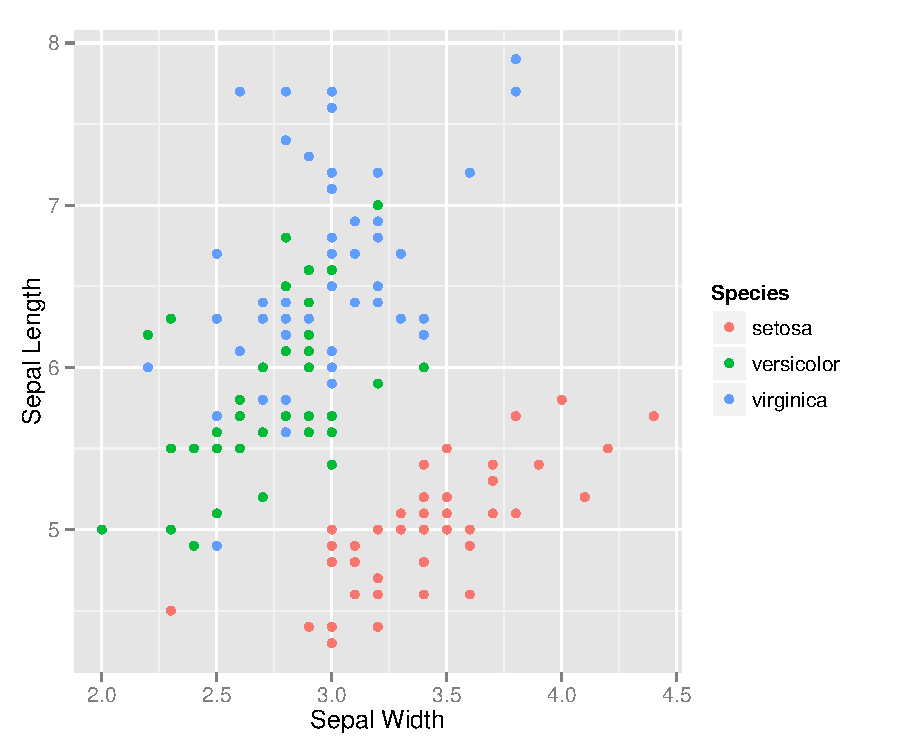
\includegraphics[width=6in,height=5in]{scatterplot.pdf}
\caption{A scatterplot of sepal width and length of iris species.}
\label{fig:scatterplot}
\end{figure}

% !Rnw root = Master.Rnw

\section{Exporting to other formats}

pandoc

online converting tool

pdftohtml

sudo apt-get install xpdf
sudo apt-get install poppler-utils % install pdftohtml

pdftohtml Master.pdf Master.html % simple results without figures or tables
pdftohtml -c Master.pdf Master.html % complex results, almost exactly the same as PDF

\begin{figure}
\centering
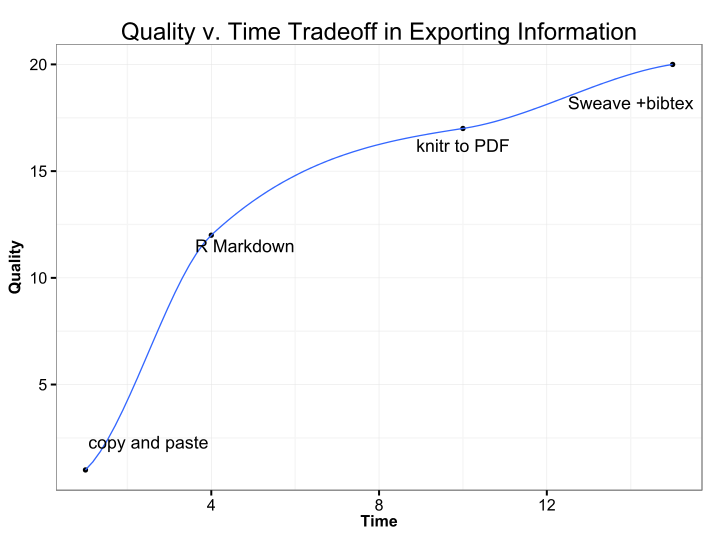
\includegraphics[width=0.8\textwidth]{qualityvstime.png}
\caption{Quality vs. Time}
\label{fig:qualityvstime}
\end{figure}

% !Rnw root = Master.Rnw

\section{Conclusions}

To appear...


\printbibliography

\end{document}
